% Digital Logic Report Template
% Created: 2020-01-10, John Miller

%==========================================================
%=========== Document Setup  ==============================

% Formatting defined by class file
\documentclass[11pt]{article}

% ---- Document formatting ----
\usepackage[margin=1in]{geometry}	% Narrower margins
\usepackage{booktabs}				% Nice formatting of tables
\usepackage{graphicx}				% Ability to include graphics

%\setlength\parindent{0pt}	% Do not indent first line of paragraphs 
\usepackage[parfill]{parskip}		% Line space b/w paragraphs
%	parfill option prevents last line of pgrph from being fully justified

% Parskip package adds too much space around titles, fix with this
\RequirePackage{titlesec}
\titlespacing\section{0pt}{8pt plus 4pt minus 2pt}{3pt plus 2pt minus 2pt}
\titlespacing\subsection{0pt}{4pt plus 4pt minus 2pt}{-2pt plus 2pt minus 2pt}
\titlespacing\subsubsection{0pt}{2pt plus 4pt minus 2pt}{-6pt plus 2pt minus 2pt}

% ---- Hyperlinks ----
\usepackage[colorlinks=true,urlcolor=blue]{hyperref}	% For URL's. Automatically links internal references.

% ---- Code listings ----
\usepackage{listings} 					% Nice code layout and inclusion
\usepackage[usenames,dvipsnames]{xcolor}	% Colors (needs to be defined before using colors)

% Define custom colors for listings
\definecolor{listinggray}{gray}{0.98}		% Listings background color
\definecolor{rulegray}{gray}{0.7}			% Listings rule/frame color

% Style for Verilog
\lstdefinestyle{Verilog}{
	language=Verilog,					% Verilog
	backgroundcolor=\color{listinggray},	% light gray background
	rulecolor=\color{blue}, 			% blue frame lines
	frame=tb,							% lines above & below
	linewidth=\columnwidth, 			% set line width
	basicstyle=\small\ttfamily,	% basic font style that is used for the code	
	breaklines=true, 					% allow breaking across columns/pages
	tabsize=3,							% set tab size
	commentstyle=\color{gray},	% comments in italic 
	stringstyle=\upshape,				% strings are printed in normal font
	showspaces=false,					% don't underscore spaces
}

% How to use: \Verilog[listing_options]{file}
\newcommand{\Verilog}[2][]{%
	\lstinputlisting[style=Verilog,#1]{#2}
}




%======================================================
%=========== Body  ====================================
\begin{document}

\title{ELC 2137 Lab 6: MUX and 7-segment Decoder}
\author{CJ Jones, Jake Simmons}

\maketitle


\section*{Summary}

This lab explored using a Basys3 board to produce an 8-bit number on a 7-segment display through a MUX combinational logic design. This lab produced a cheat button that turns the display from hex to decimal, and back because of the difficulty of reading the decimal numbers. Using Verilog, some skills gained in this lab include: writing a multiplexer utilizing the conditional operator, use the double-dabble algorithm to convert hex values into BCD, using multi-bit signals, using constraint files,and creating a design on a FPGA board. Overall, this lab demonstrated how to utilize software and programmable logic to produce a hardware output.








\section*{Results}


\begin{figure}[ht]\centering
	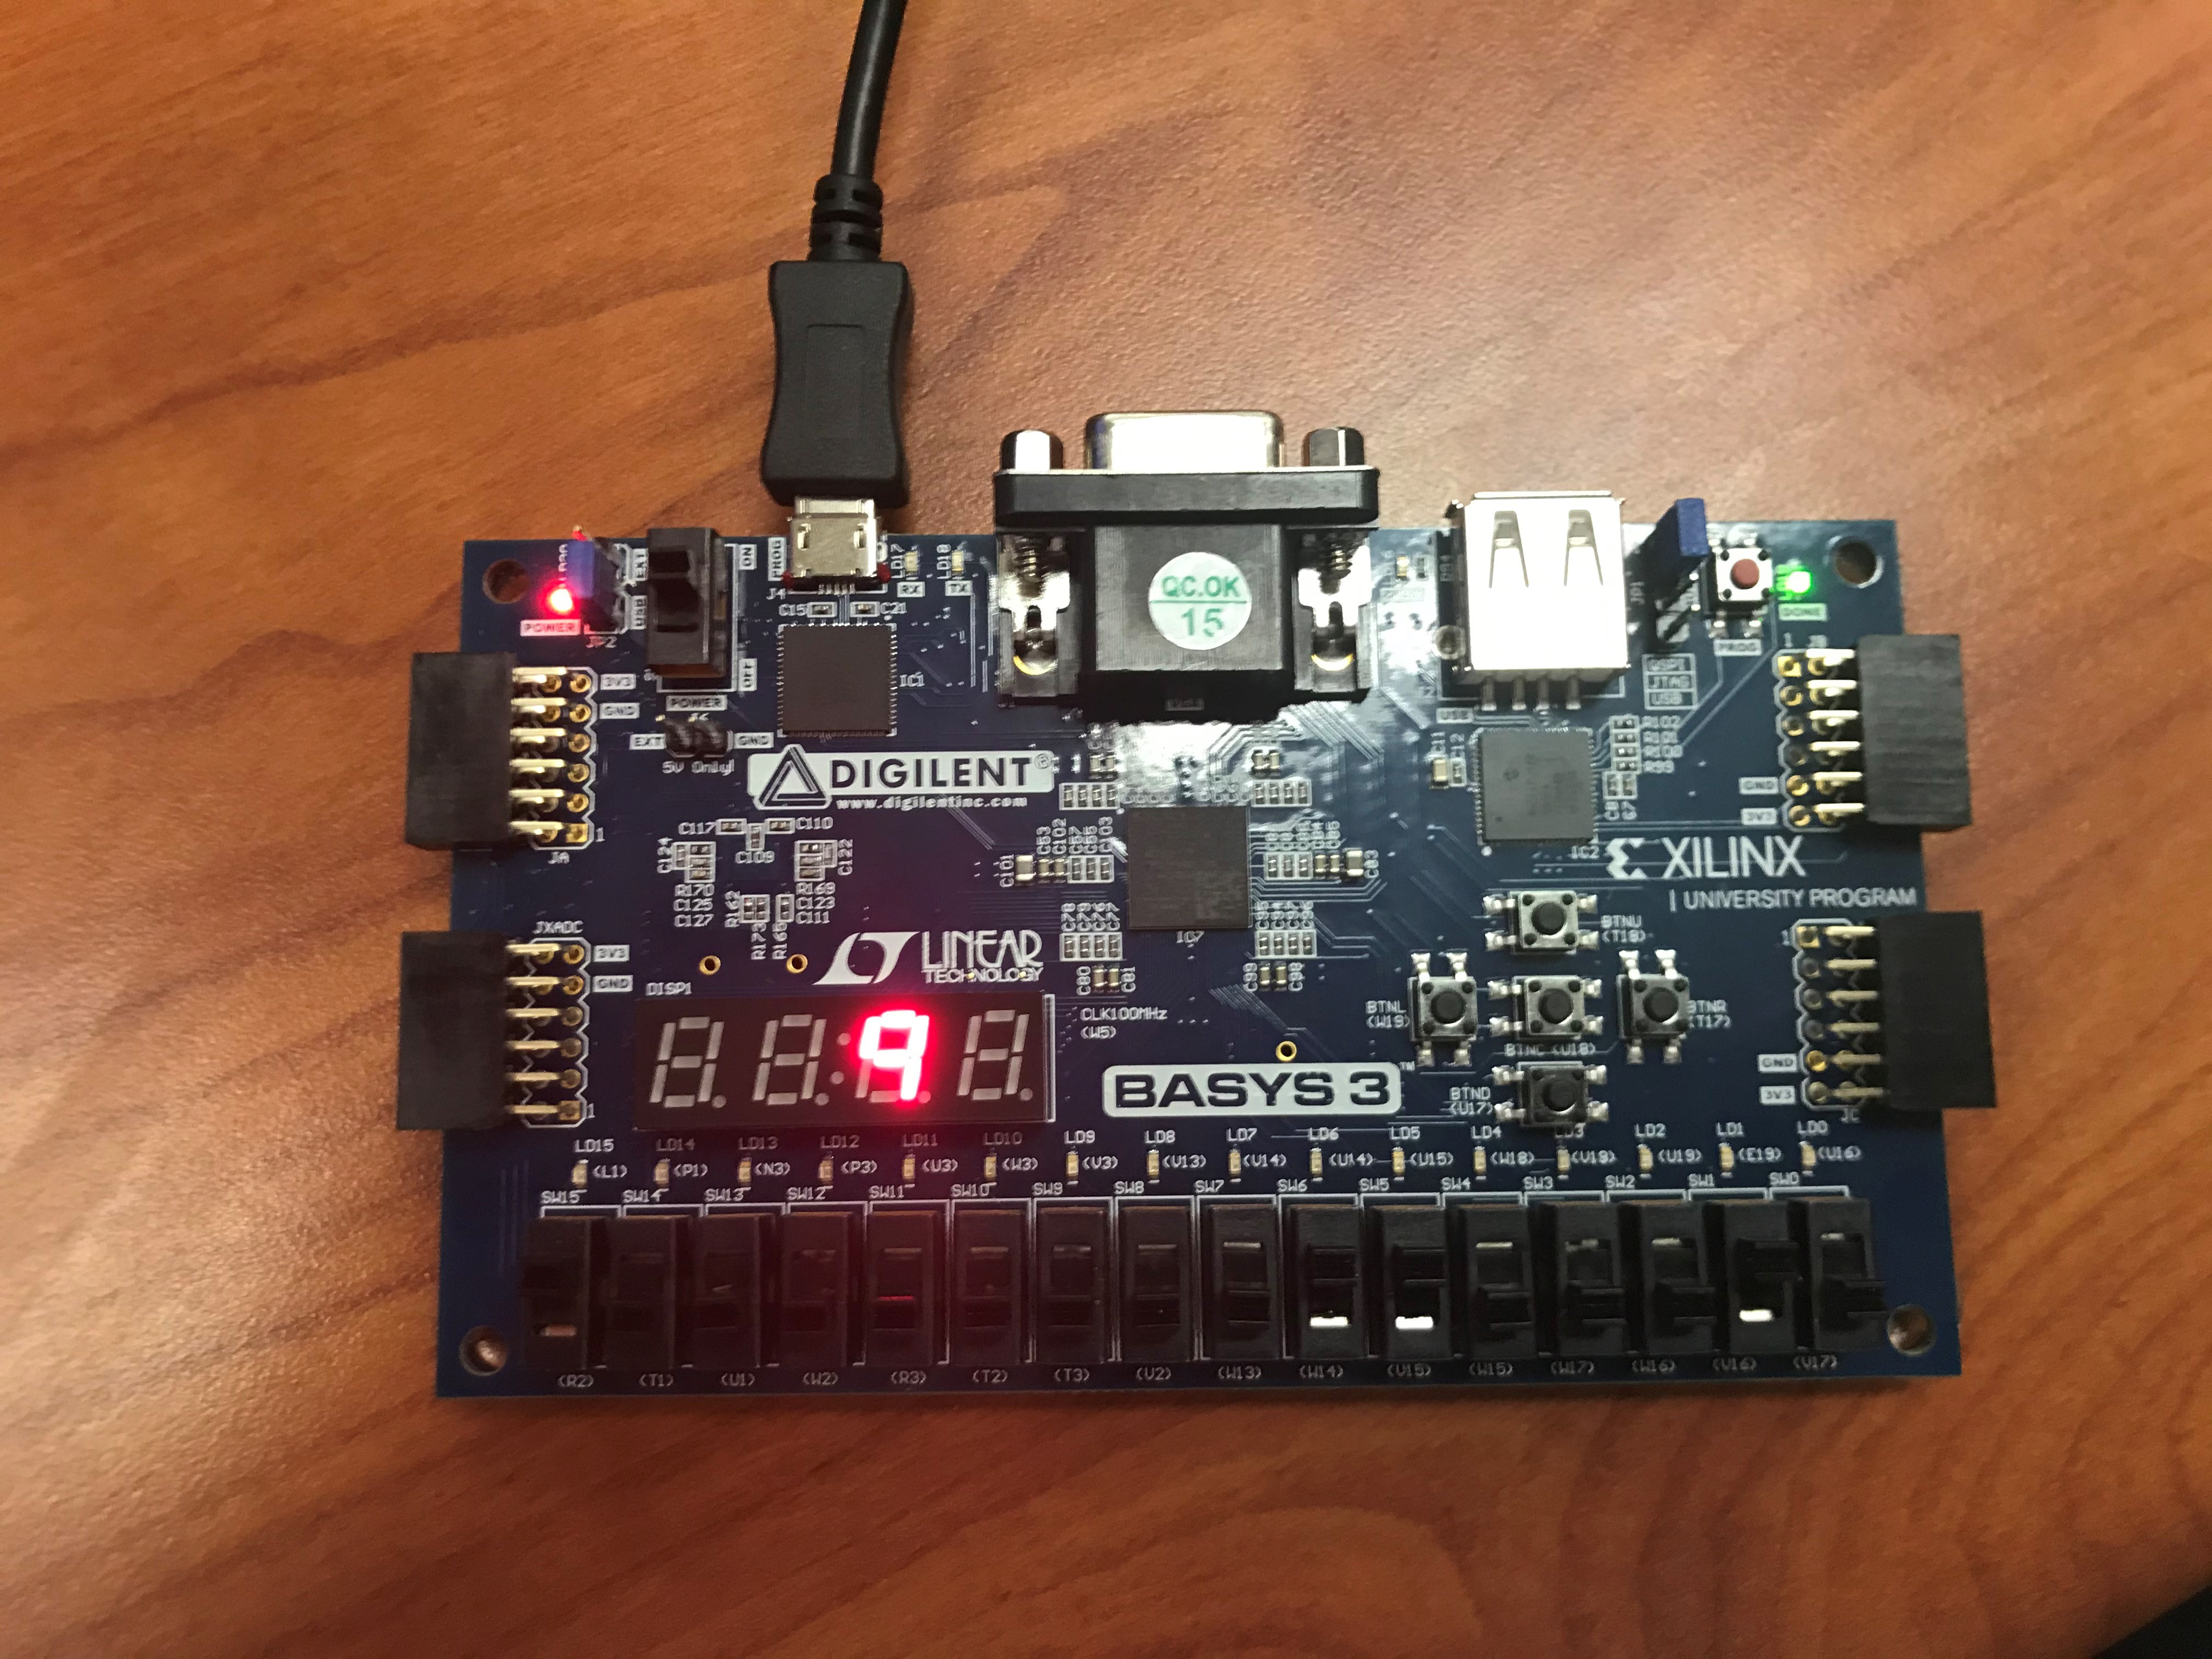
\includegraphics[width=1.0\textwidth]{9}
	\caption{Picture of board}
	\label{fig:sim_with_table}
\end{figure}

\begin{figure}[ht]\centering
	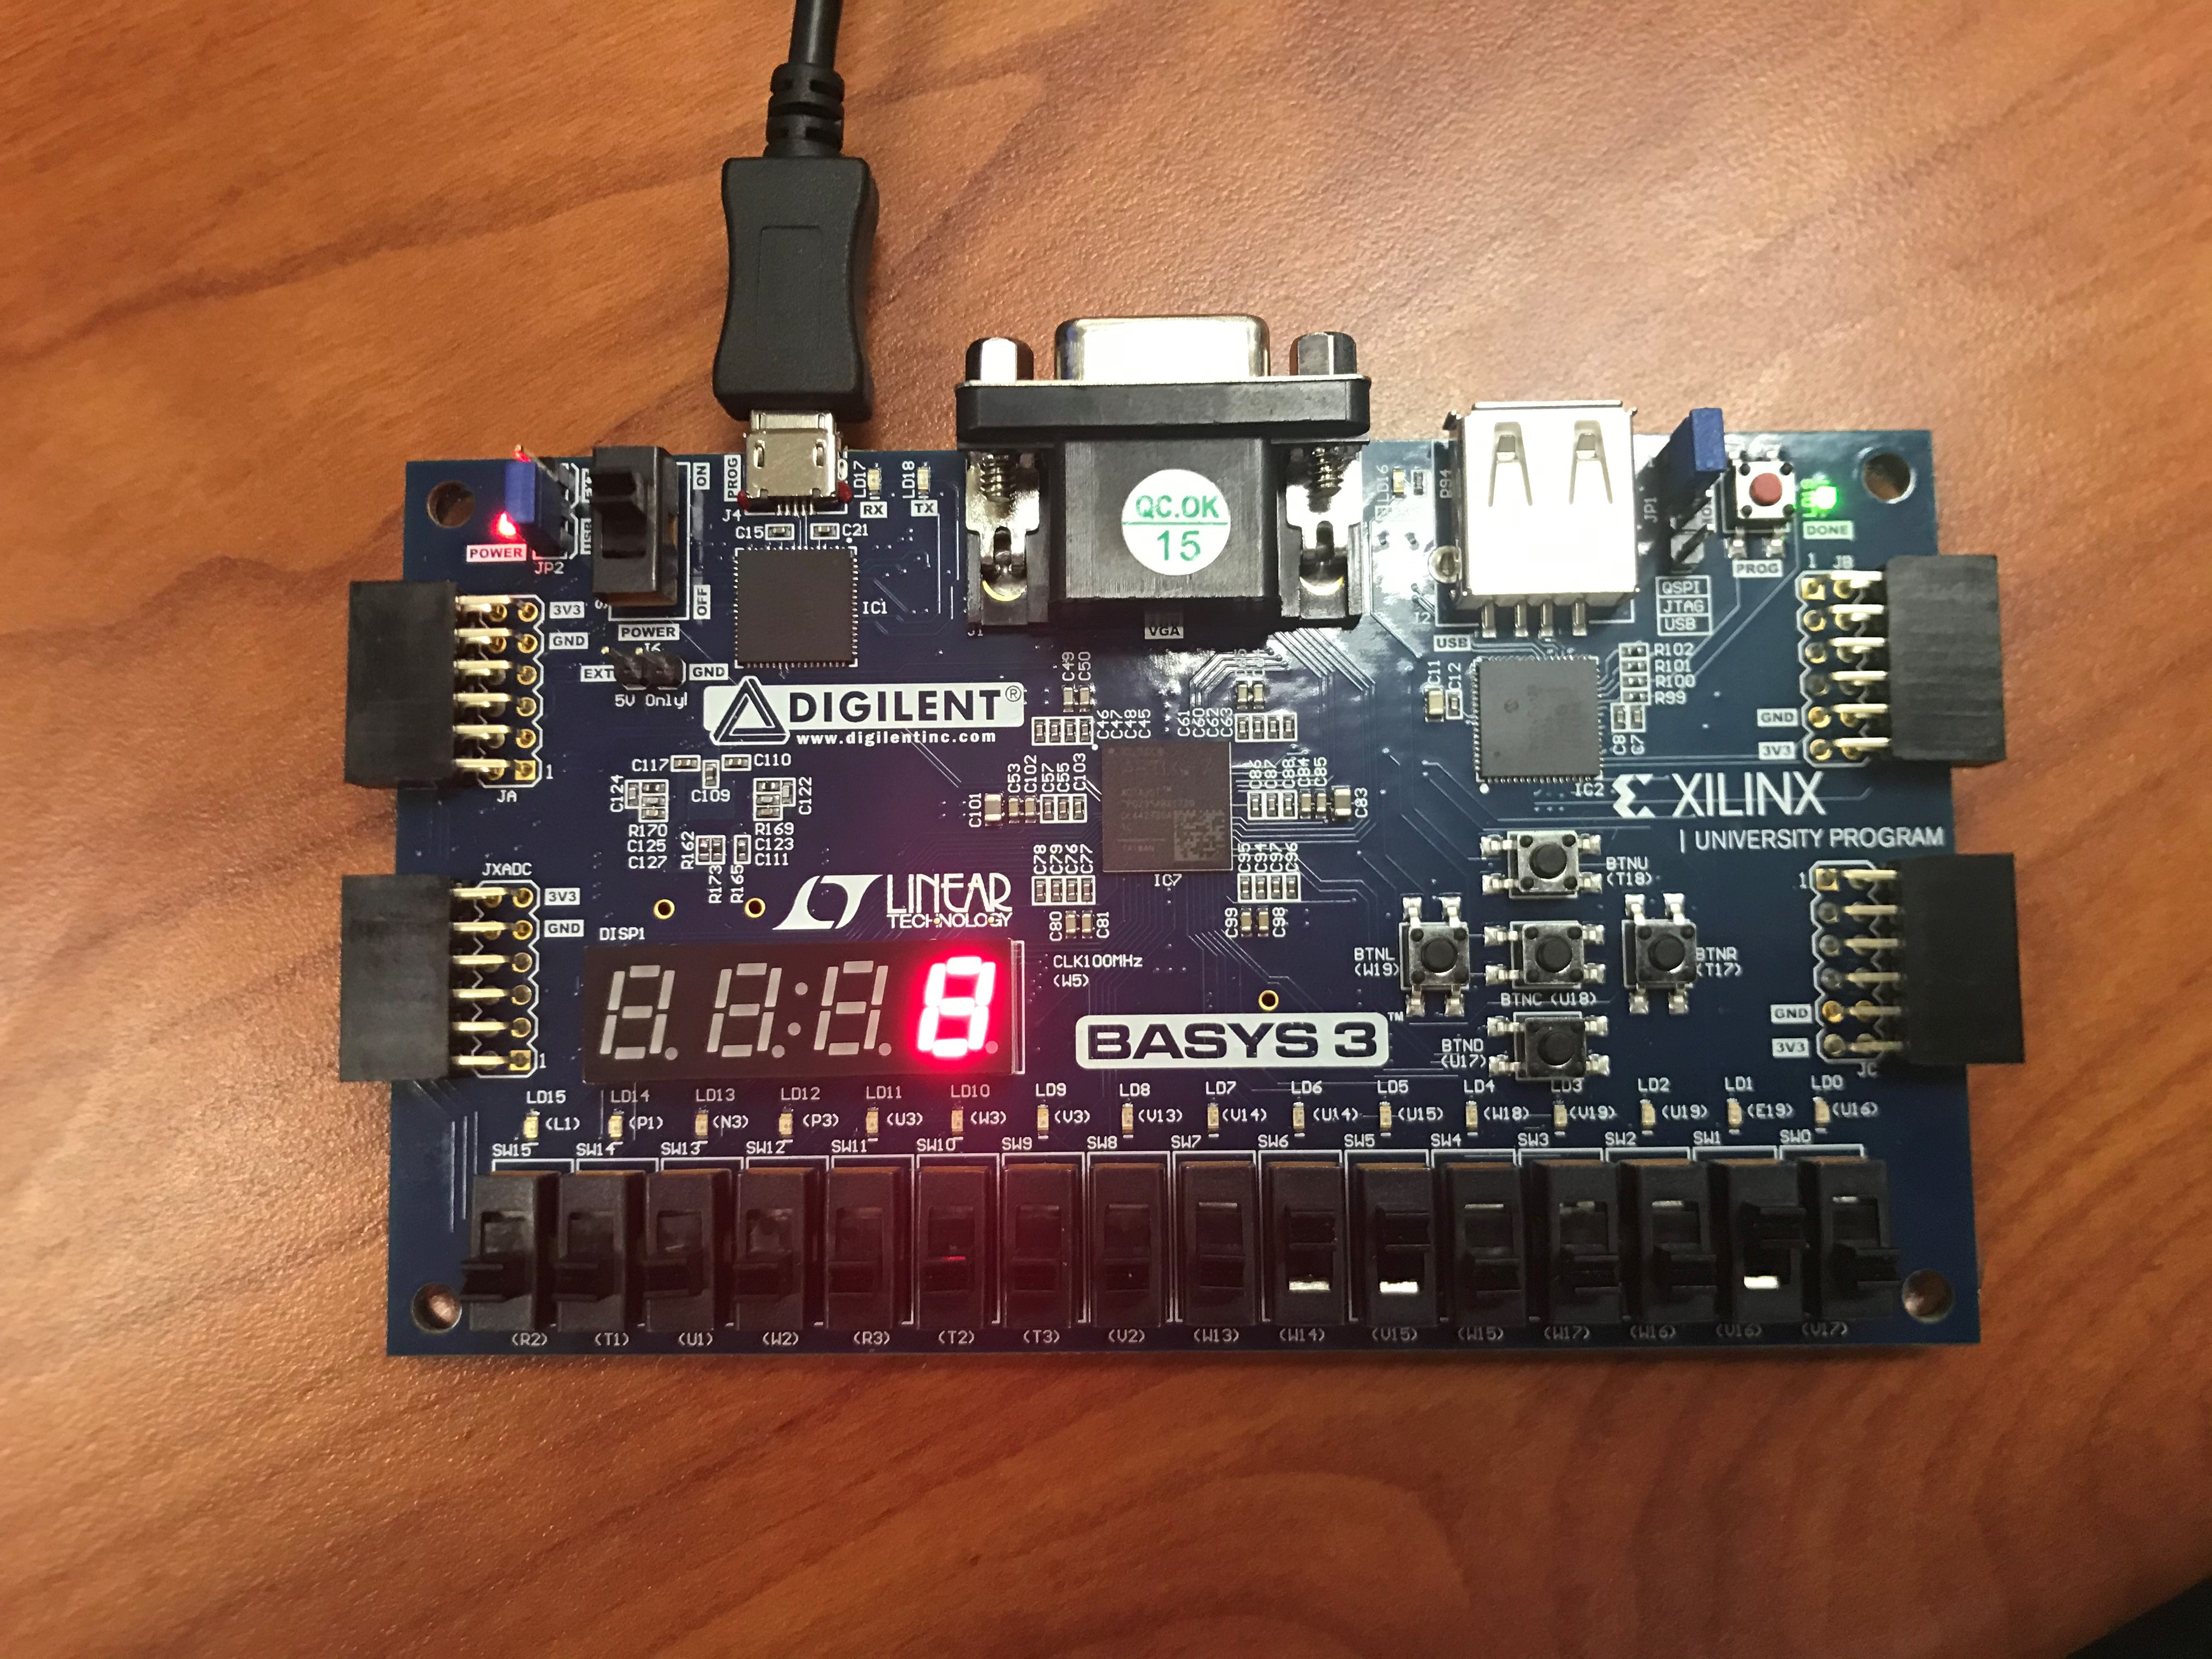
\includegraphics[width=1.0\textwidth]{8}
	\caption{Picture of Board}
	\label{fig:sim_with_table}
\end{figure}


\begin{figure}[ht]\centering
	\begin{tabular}{l|rrrrrrrrrrrrrrr}
		Time (ns): & 0 & 10 & 20 & 30 & 40 & 50 & 60 & 70 & 80 & 90 & 100 & 110 & 120 & 130 & 140 \\
		\midrule 
		B & 0 & 1 & 2 & 3 & 4 & 5 & 6 & 7 & 8 & 9 & a & b & c & d & e \\
		O & 0 & 1 & 2 & 3 & 4 & 8 & 9 & a & b & c & d & e & f & 0 & 1\\
		
		 
	\end{tabular}\medskip
	
	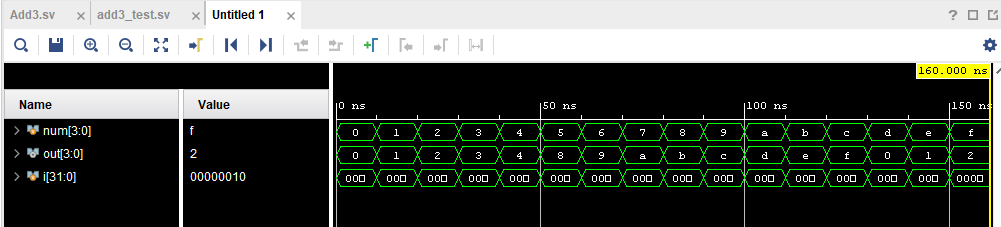
\includegraphics[width=1.0\textwidth]{Add3WaveForm}
	\caption{Add3 simulation waveform and ERT}
	\label{fig:sim_with_table}
\end{figure}

\begin{figure}[ht]\centering
	\begin{tabular}{l|rrrrrr}
		Time (ns): & 0 & 10 & 20 & 610 & 620 & 630 \\
		\midrule 
		Input & 0 & 1 & 2 & 3c & 3d & 3e \\
		Output & 0 & 1 & 2 & 60 & 61 & 62 \\
	\end{tabular}\medskip
	
	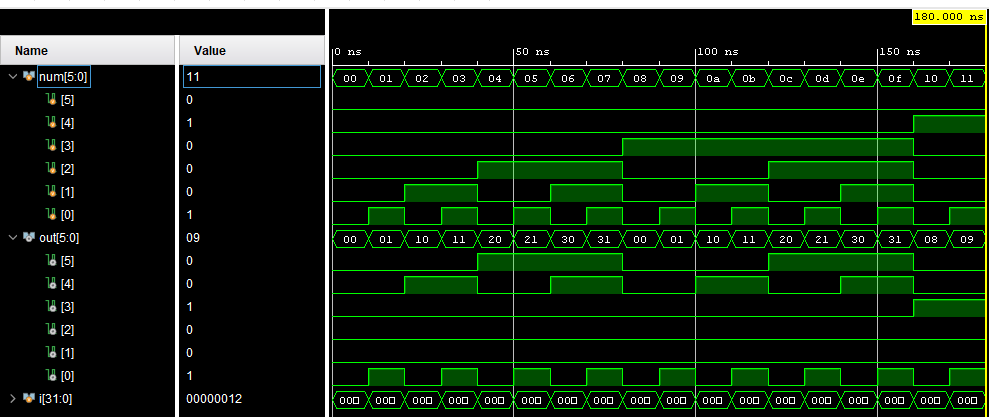
\includegraphics[width=1.0\textwidth]{Part2}
	\caption{BCD6 simulation waveform and ERT}
	\label{fig:sim_with_table}
\end{figure}

\begin{figure}[ht]\centering
	\begin{tabular}{l|rrrrrr}
		Time (ns): & 0 & 10 & 20 & 970 & 980 & 990 \\
		\midrule 
		Input & 0 & 1 & 2 & 61 & 62 & 63 \\
		Output & 0 & 1 & 2 & 897 & 898 & 899 \\
	\end{tabular}\medskip
	
	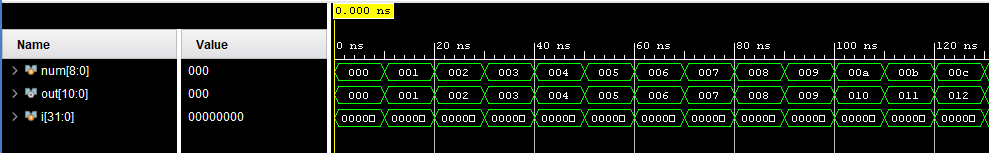
\includegraphics[width=1.0\textwidth]{11BitFirst}
	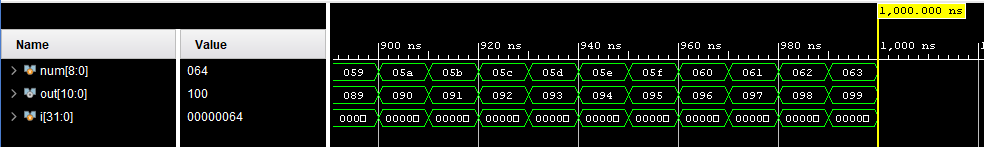
\includegraphics[width=1.0\textwidth]{11BitSecond}
	\caption{BCD11 simulation waveform and ERT}
	\label{fig:sim_with_table}
\end{figure}


\begin{figure}[ht]\centering
	
	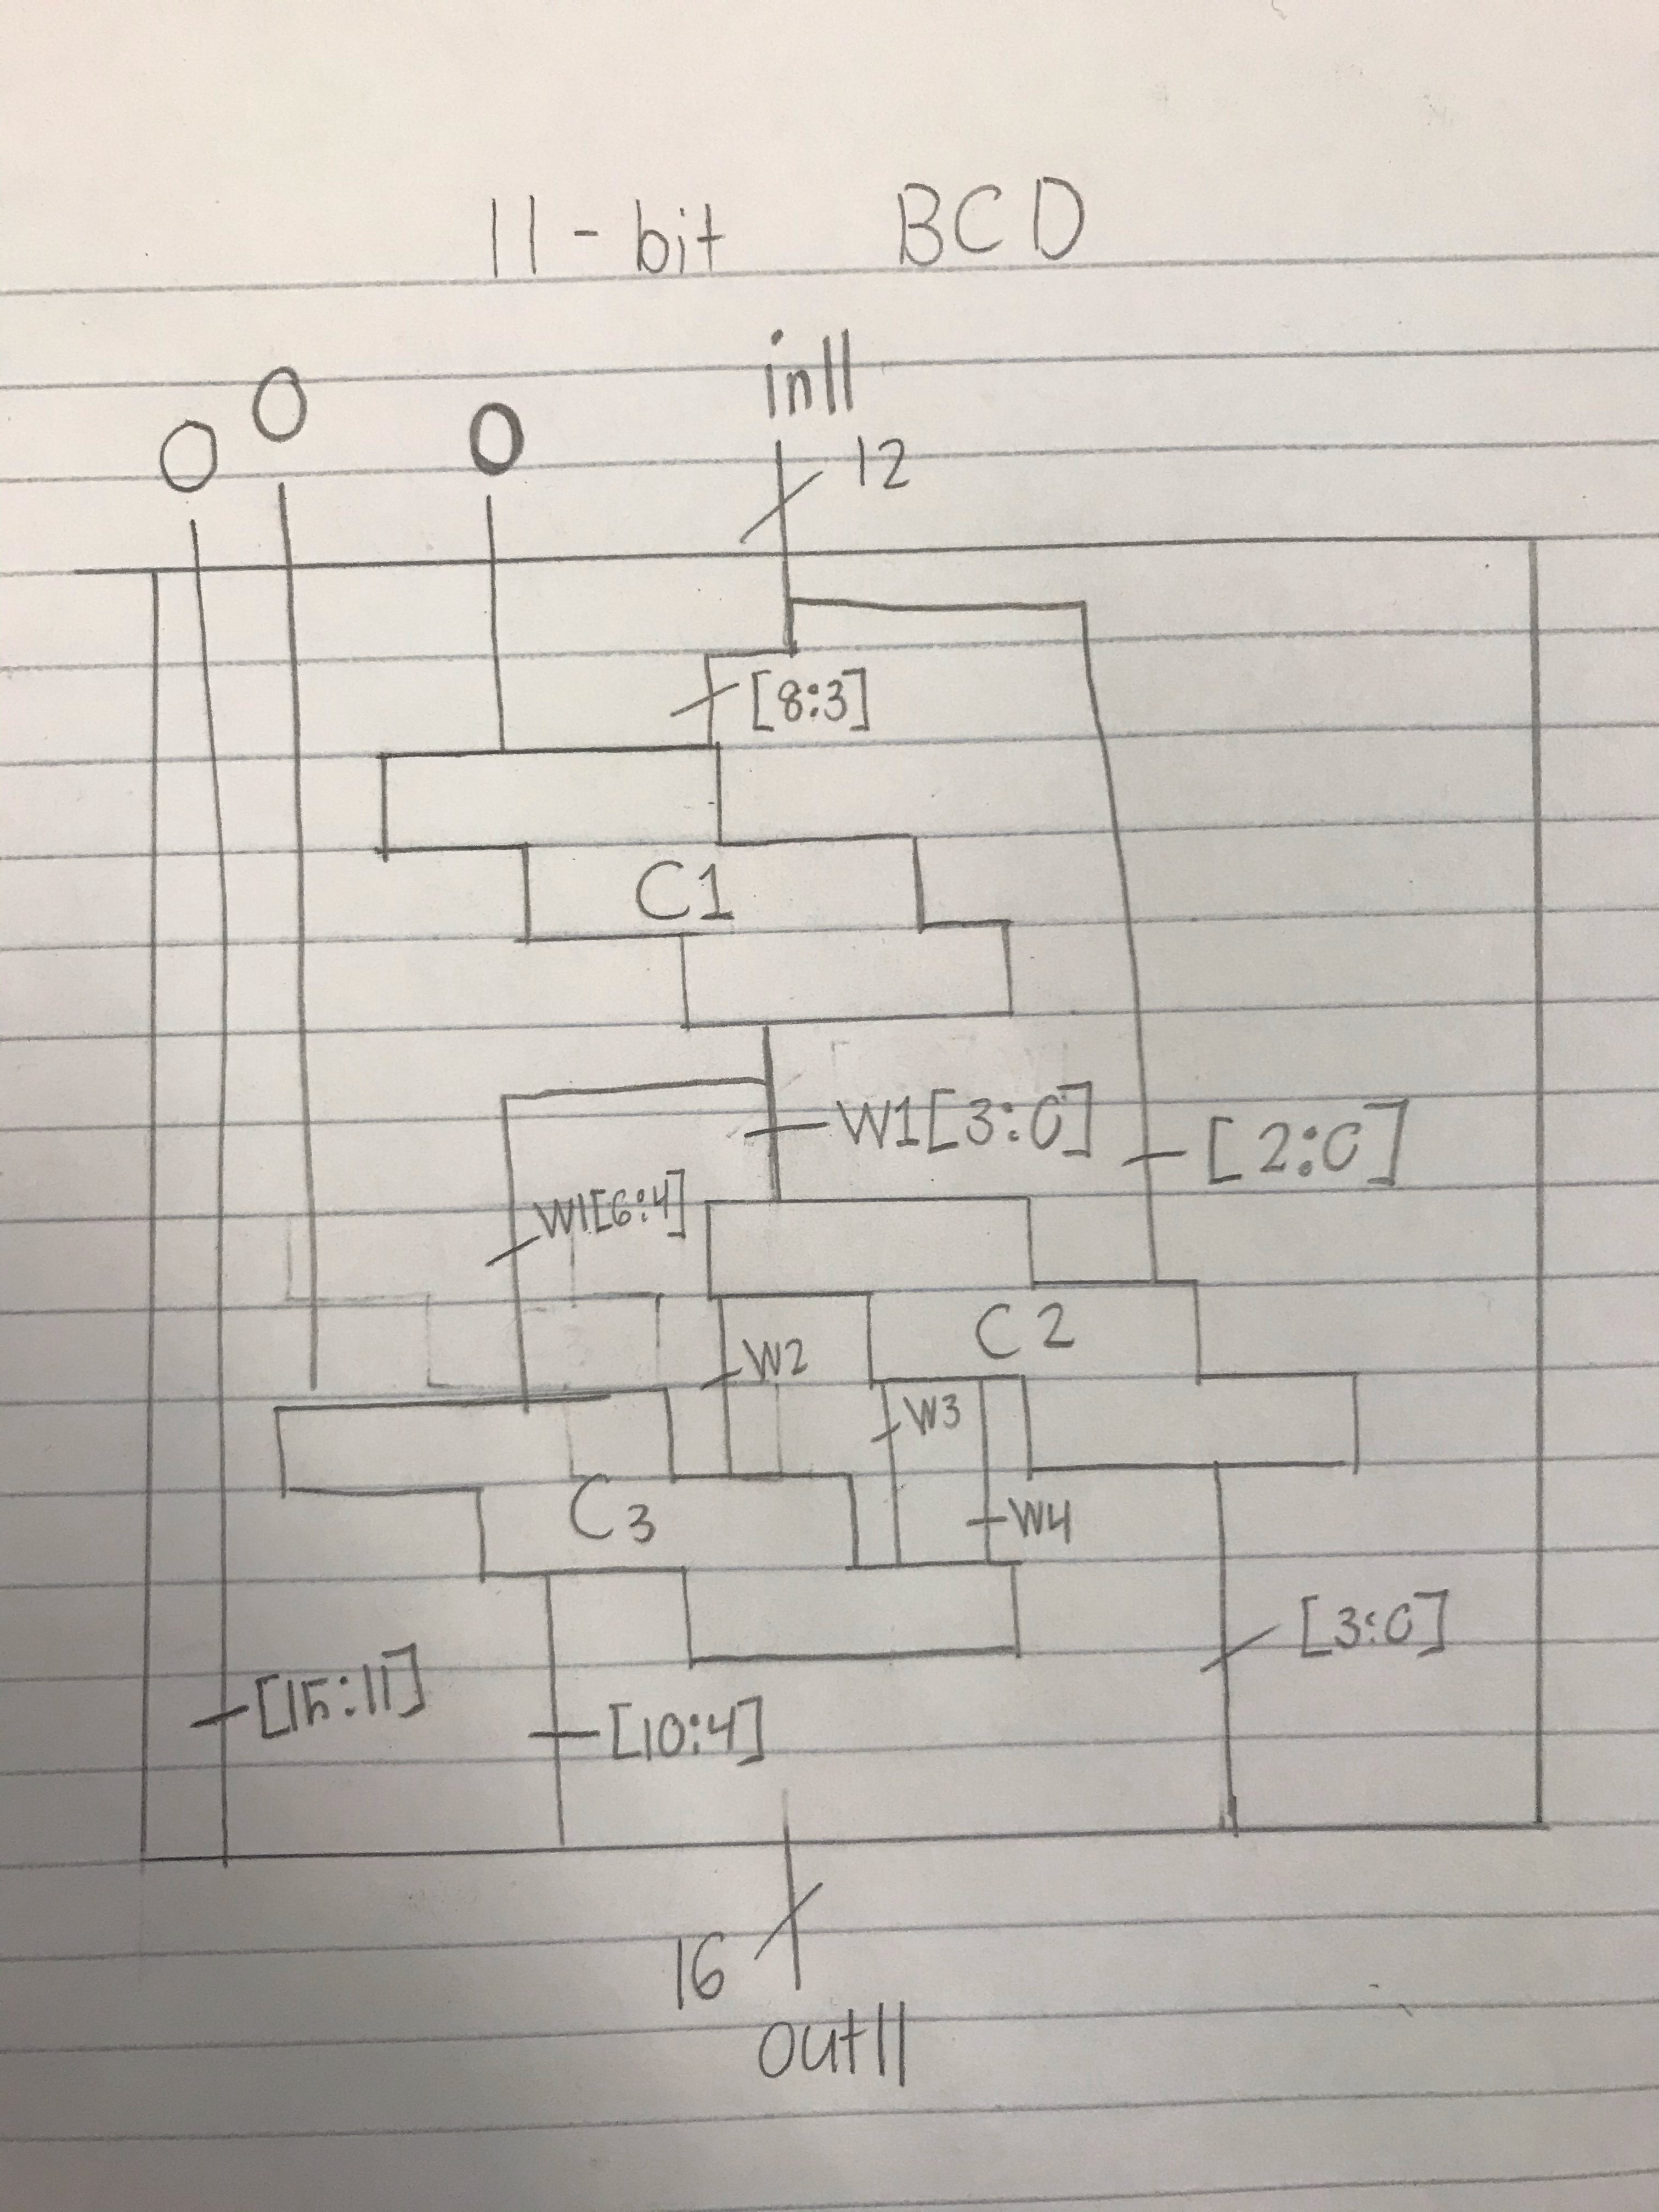
\includegraphics[width=1.0\textwidth]{Circuit Diagram}
	\caption{Circuit Diagram}
	\label{fig:sim_with_table}
\end{figure}
\clearpage


\section*{Code}

\begin{lstlisting}[style=Verilog,caption=Add3 Module Code,label=code:ex ]

// Jake Simmons and Chris Jones , ELC 2137, 2020 -3-24

module add3(
input  [3:0] Cin,
output reg [3:0] Cout);

always @*
begin
if (Cin > 4'd4)
Cout = Cin + 4'd3;
else
Cout = Cin;
end

endmodule //Add3


\end{lstlisting}



\begin{lstlisting}[style=Verilog,caption=Add3 Testbench Code,label=code:ex ]

// Jake Simmons and Chris Jones , ELC 2137, 2020 -3-24

module add3_test () ;

	  reg [3:0] num;
	  
	  wire [3:0] out;
	  
	  integer i ; // Declare loop variable
	  
	  
	  Add3 C1 (.Cin(num), .Cout(out));
	  
	  
	  
	  initial begin
	  
	  for ( i =0; i <=8'hF ; i = i +1) begin
	  
	  num = i;
	  
	  #10;
	  
	  end
	  
	  $finish ;
	  
	  end
	  
	  endmodule // sseg_decoder_test
	  



\end{lstlisting}



\begin{lstlisting}[style=Verilog,caption=BCD6 Module Code,label=code:ex ]

// Jake Simmons and Chris Jones , ELC 2137, 2020 -3-24
module BCD6(
input [6:0] B,
output [6:0] Out
);
wire W1, W2, W3;
wire W4, W5, W6;

Add3 C1(.Cin(B[6:3]), .Cout({ Out[6],W3 , W2, W1}));

Add3 C2(.Cin({W3,W2,W1,B[2]}), .Cout({Out[5],W4,W5,W6}));       

Add3 C3(.Cin({W4,W5,W6,B[1]}), .Cout({Out[4], Out[3], Out[2], Out[1]}));

assign Out[0] = B[0];

endmodule

\end{lstlisting}



\begin{lstlisting}[style=Verilog,caption=BCD6 Test Bench Code,label=code:ex ]
// Jake Simmons and Chris Jones , ELC 2137, 2020 -3-24

module BCD6_Test () ;

reg [5:0] num;

wire [5:0] out;

integer i ; // Declare loop variable


BCD6 BCD (.B(num), .Out(out));



initial begin

for ( i =0; i <=6'h111111 ; i = i +1) begin

num = i;

#10;

end

$finish ;

end

endmodule // sseg_decoder_test


\end{lstlisting}



\begin{lstlisting}[style=Verilog,caption=BCD11 Module Code,label=code:ex ]
// Jake Simmons and Chris Jones , ELC 2137, 2020 -3-24

module BCD11(
input [11:0] in11,
output [15:0] out11
);

wire [6:0] W1;
wire W2, W3, W4;
BCD6 C1( .B({0, in11[8:3]}), .Out(W1)
);

BCD6 C2( .B({W1[3:0], in11[2:0]}), .Out({W2, W3, W4,out11[3:0]})
);

BCD6 C3( .B({0,W1[6:4], W2, W3, W4}), .Out(out11[10:4])
);
assign out11[15:11] = 0;
endmodule


\end{lstlisting}

\begin{lstlisting}[style=Verilog,caption=BCD11 Test Bench Code,label=code:ex ]
// Jake Simmons and Chris Jones , ELC 2137, 2020 -3-24

module BCD11_Test () ;

reg [8:0] num;

wire [10:0] out;

integer i ; // Declare loop variable


BCD11 BCD (.in11(num), .out11(out));



initial begin

for ( i =0; i <=9'h111111111 ; i = i +1) begin

num = i;

#10;

end

$finish ;

end

endmodule // sseg_decoder_test



\end{lstlisting}

\begin{lstlisting}[style=Verilog,caption=sseg1 module Code,label=code:ex ]
// Jake Simmons and Chris Jones , ELC 2137, 2020 -3-24

module sseg1(
input [15:0] sw,
output [3:0] an,
output [6:0] seg,
output dp
);

wire [3:0] muxwire;
wire [7:0] W1; 

BCD11 BD11(
.in11(sw[10:0]), .out11(W1));

mux2_4b m1(
.in1(W1[7:4]), .in0(W1[3:0]),
.sel(sw[15]), .out(muxwire[3:0])
);

sseg_decoder sseg1(
.sseg(seg), .num(muxwire[3:0])
);

assign an[3:2] = 3;
assign dp = 1;
assign an[1] = ~sw[15];
assign an[0] = sw[15];
endmodule



\end{lstlisting}





\end{document}

